It was Monday and, as usual, Liz was waiting for Emily and Charlie to turn up at the entrance to the school. But this time, standing on the stone steps, she was more anxious than normally.

And then she saw the familiar blond haircut from afar. She ran down the steps to meet up with her friends sooner.

“Liz!” Emily exclaimed and embraced her best friend with a weak smile on her face.

“I saw the news!” the redhead told her.

“What news?”

“That you and Charlie went into the haunted house and it was set on fire!” she explained, “Where is Charlie, by the way? Is he okay?”

“Erm, well, physically yes. Mentally—not so much…”

“What happened?!”

“Matthew set it on fire,” she said curtly, “And Charlie's neighbor perished…”

“Oh. I'm really sorry… Gosh, that's horrifying… Are you okay?”

“I guess…”

Liz hugged her one more time, and they started walking up the steps slowly. But the red-haired girl stopped suddenly before going in through the door.

“What is it?” Emily asked, coming to a halt in front of her and turning around.

“Can you tell me where Charlie is, please?”

“At his neighbor's. Says he doesn't want to see anybody… Why?”

“What house is that?”

“I don't remember the number, but the blue one next to his,” Emily stated, confused, “Why?”

“I have to go,” Liz said and ran down the stairs.

“Wait!” Emily called, “Go where? The bell is about to ring!”

“I hope you don't mind, love you, bye!” she cried back and sprinted towards the given location.

\bigskip

Charlie was sitting on what used to be Mr. Brown's floor. The blinds of the hallway windows were closed, as well as the curtain of the small window on the front door.

Before the boy lay letters, spread about the carpet. He was just putting one down to read the other—they were letters for Mr. Brown's wife that he had never sent—when the doorbell rang.

He furrowed his eyebrows: the first lesson was about to begin and he specifically told Emily he didn't want to see her, or anybody for that matter. But nevertheless he got up from the floor and walked over to the front door in a quiet manner. He pulled the curtain away a bit and looked through the dirty window. It was Liz. He opened the door in surprise and confusion.

“Hi!” she exclaimed with a smile.

“Hi?” he replied.

“Do you mind if I come in?”

He opened the door further into the house for her. She stepped over the threshold with a soft smile.

“What are you doing here?” he asked as she seated herself on the floor among the letters.

“Visiting you,” she said and patted the carpet for him to sit down.

He hesitated, but did as she gestured: he hadn't expected her to come.

“Shouldn't you be in class?” he questioned in the same tone he usually did.

“Well, you skipped class for me, so I skipped class for you.”

“Oh,” he smiled at her faintly, “Thank you.”

“That's what friends do, right?” she shrugged carelessly like she wouldn't be grounded for skipping school afterwards.

Then, they sat in silence for a good amount of time. But it wasn't that sort of uncomfortable silence. It was the kind of silence that spoke louder than words ever could.

During this silence they looked around the hallway and through the letters until Liz broke it.

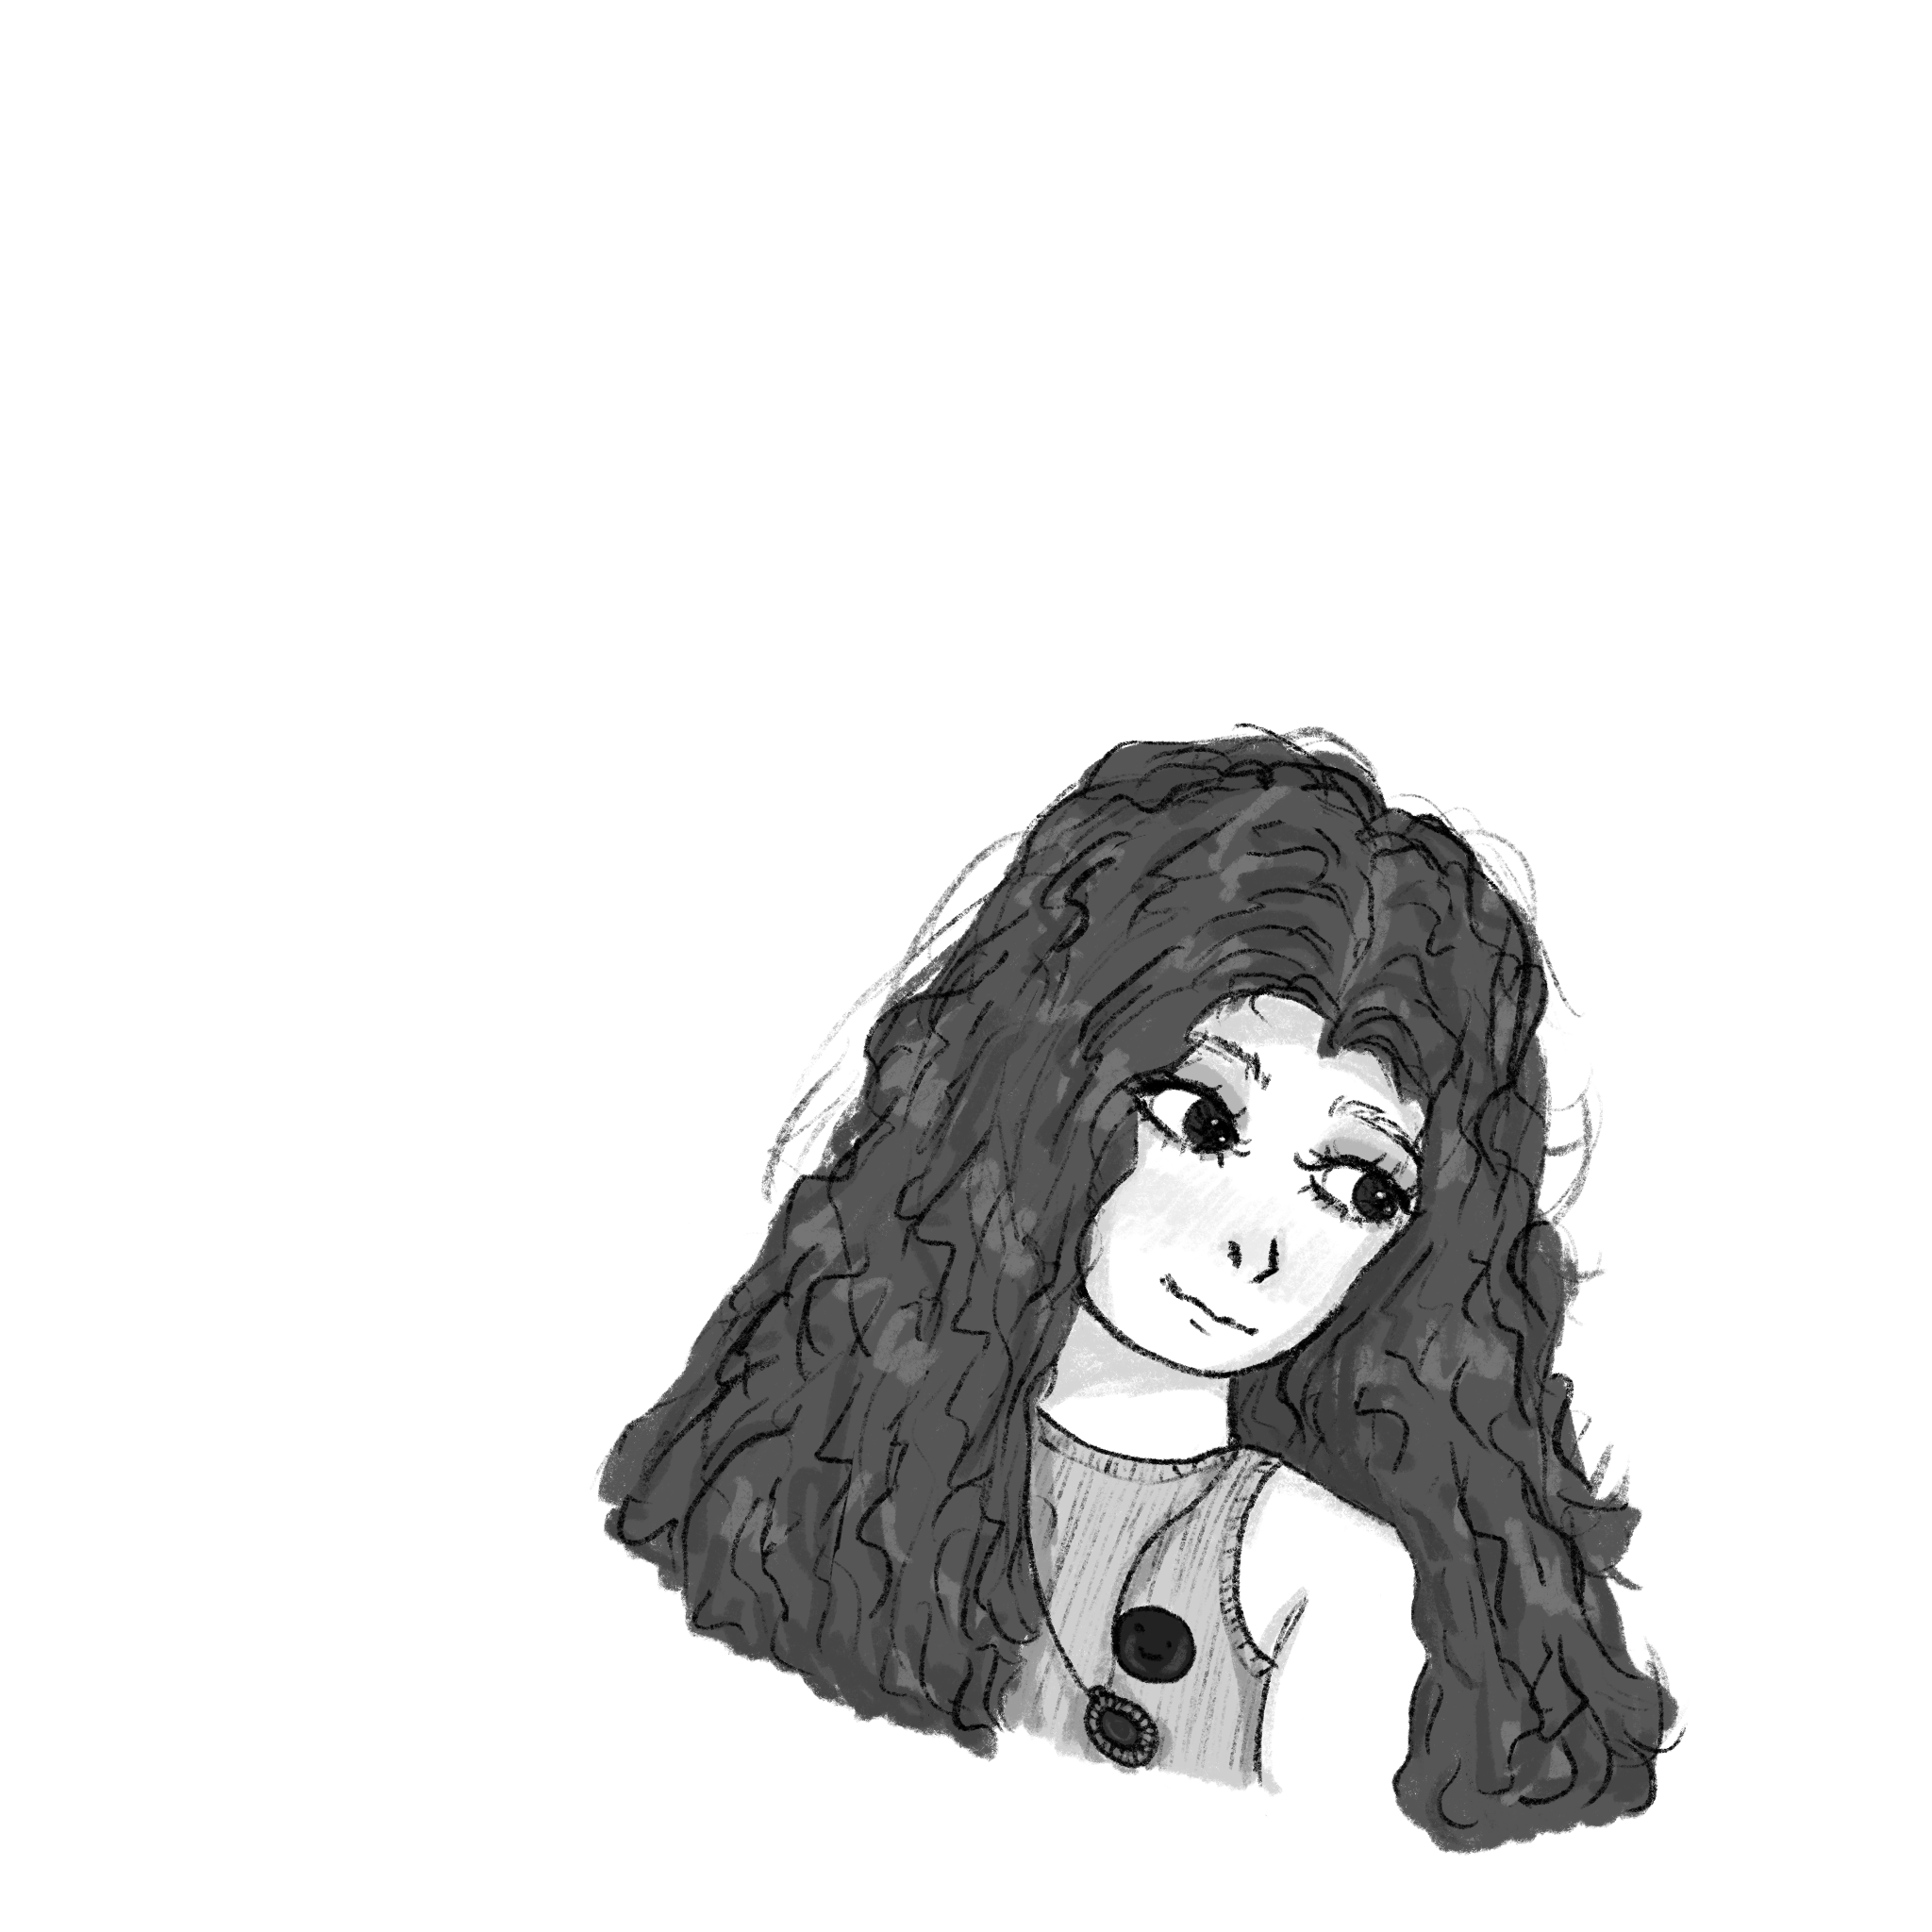
\includegraphics[width=0.99\textwidth]{Liz.png}

“You know…” she started.

“Yeah?”

“I think I can feel his spirit here.”

“In the hallway?” Charlie half-smiled.

“No, in this,” she gestured to what they were doing. “In the silence, in the atmosphere.”

“Have you even met him?” he asked with a chuckle.

“You don't have to meet people to feel their spirit,” she informed sternly.

Charlie straightened his back and nodded with a smile.

Then there was silence once more.

“You know what?” he started this time.

“Yeah?”

“I think you're right. I can feel him too.”

They smiled and the silence continued. They were communicating through gestures while shuffling through the letters together. And then, while pointing to a word in a letter, Charlie froze for a second.

“So did you find out what that was?” he broke the silence this time.

“What what was?” she questioned in confusion.

“The thing you are going through with Lillian?”

“Oh,” she said, dropping a letter onto the floor, “Well, I think I might be aromantic.”

“What's that?”

“Well, there are different kinds, apparently. And I, personally, get second-hand embarassment from romance and all that stuff, basically.”

“Have you told Lillian about it?”

“No, I mean, I'm still not sure… I've only been researching for like three days.”

“You'll figure it out, I know you will,” he smiled, “I can help you if you want.”

“Thank you,” she smiled back at him.

“That's what friends do, right?” he gave a shrug just like the one she had given him.

And they continued looking through all the letters, eventually moving on to the living room from the hall. And all in pure silence. The purest silence you could find.